\chapter{智慧煤矿发展现状与展望:\\ 基于数字孪生与平行系统的文献综述}

\section{研究背景}

煤炭作为我国的基础能源,其安全、高效与绿色的开采对于保障国家能源安全具有不可替代的战略意义。近年来,随着浅部煤炭资源的日益枯竭,煤矿开采不可避免地向深部地层延伸。深部开采伴随的高地应力、高瓦斯、高地温以及复杂的岩溶水文地质条件,使得煤与瓦斯突出、冲击地压等重特大动力灾害的防控难度急剧上升。传统的煤矿开采模式受限于高危作业环境以及粗放型的人工管理方式,已难以满足现代工业对于本质安全与生产效率的升级需求。在这一宏观背景下,煤矿智能化建设应运而生,并迅速成为应对深部开采挑战与实现煤炭工业高质量发展的核心技术支撑 \citep{WangGuoFa_MeiKuangZhiNengHuaMeiTanGongYeGaoZhiLiangFaZhanDeHeXinJiShuZhiCheng_2019}。

早期的智慧煤矿探索主要集中在底层设备的单机自动化改造与基础信息系统的建设,旨在实现机电设备的远程启停与初步的工况参数监测 \citep{WangGuoFa_ZhiHuiMeiKuangYuZhiNengHuaKaiCaiGuanJianHeXinJiShuFenXi_2019}。然而,这种基于逻辑可编程控制器与工业组态软件的系统缺乏全局数据交互与协同规划能力。面对井下瞬息万变的地质异常与突发生产状况,孤岛式的控制单元无法形成有效的多系统联动。为了突破这一系统性瓶颈,学术界和工业界开始引入工业物联网、第五代移动通信技术、大数据分析以及新一代人工智能算法,推动矿山信息化向具备深度感知与自主决策能力的智慧化演进。

在这一演进过程中,数字孪生作为连接物理实体与虚拟数字空间的桥梁,成为构建智慧煤矿的关键共性技术 \citep{DingEnJie_KuangShanXinXiHuaFaZhanJiYiShuZiLuanShengWeiHeXinDeZhiHuiKuangShanGuanJianJiShu_2023}。该技术不仅能够对物理矿山的三维几何空间、设备运行状态及生产全流程进行高精度的全息映射,还能依托孪生计算体进行多物理场仿真推演与反向闭环控制。从单点自动化的初级阶段迈向以数字孪生为核心的全局智慧矿山,不仅是技术工具的简单迭代,更是煤炭开采范式向数据驱动与虚实互动演进的重要标志。

\section{研究现状}

当前关于智慧煤矿的研究呈现出多学科深度交叉、从宏观体系架构到微观物理执行高度协同的显著特征。现有文献的研究脉络主要可归纳为顶层设计、数据基座构建、孪生理论拓展以及底层设备协同控制等核心维度。

\subsection{顶层设计与标准体系构建}
智慧煤矿是一个涉及人、机、环、管多维复杂要素的巨系统。缺乏统一的顶层设计和标准数据接口将直接导致系统间的数据壁垒与协同障碍。为此,研究人员率先从宏观层面确立了规范化的建设框架。王国法等深入剖析了煤矿智能化标准体系的架构与建设思路,为后续各类异构智能装备的接入与多源数据的互联互通奠定了标准化基础 \citep{WangGuoFa_MeiKuangZhiNengHuaBiaoZhunTiXiKuangJiaYuJianSheSiLu_2020}。在具体的方法论指导上,张帆等系统性地综述了智慧矿山数字孪生技术,进一步明确了矿山数字孪生的构建方法与演化机理,并指出数字孪生必须经历从几何维度的结构映射到物理维度的机理映射,再到行为维度的动态映射这一递进演化过程 \citep{ZhangFan_ZhiHuiKuangShanShuZiLuanShengJiShuYanJiuZongShu_2020, ZhangFan_KuangShanShuZiLuanShengGouJianFangFaYuYanHuaJiLi_2023},如图 \ref{fig:pic1} 为其构建的智采工作面数字孪生演化实例。鲍久圣等针对矿山环境的空间特殊性与时变复杂性,提出了矿山数字孪生模型架构,详细阐述了支撑该架构所需的高效感知网络与虚实交互关键技术 \citep{BaoJiuSheng_KuangShanShuZiLuanShengMiDTMoXingJiaGouGuanJianJiShuJiYanJiuZhanWang_2023}。邢震的最新研究综述进一步表明,面向智能矿山的数字孪生技术正加速从前期的理论架构探讨向深层次的工业现场应用落地推进 \citep{XingZhen_MianXiangZhiNengKuangShanDeShuZiLuanShengJiShuYanJiuJinZhan_2024}。

\begin{figure}[htbp]
    \centering
    % 【核心修改】直接插入你刚才手动生成的高清 PDF 文件
    % width=0.8\textwidth 表示让图片宽度占据页面文本宽度的 80%
    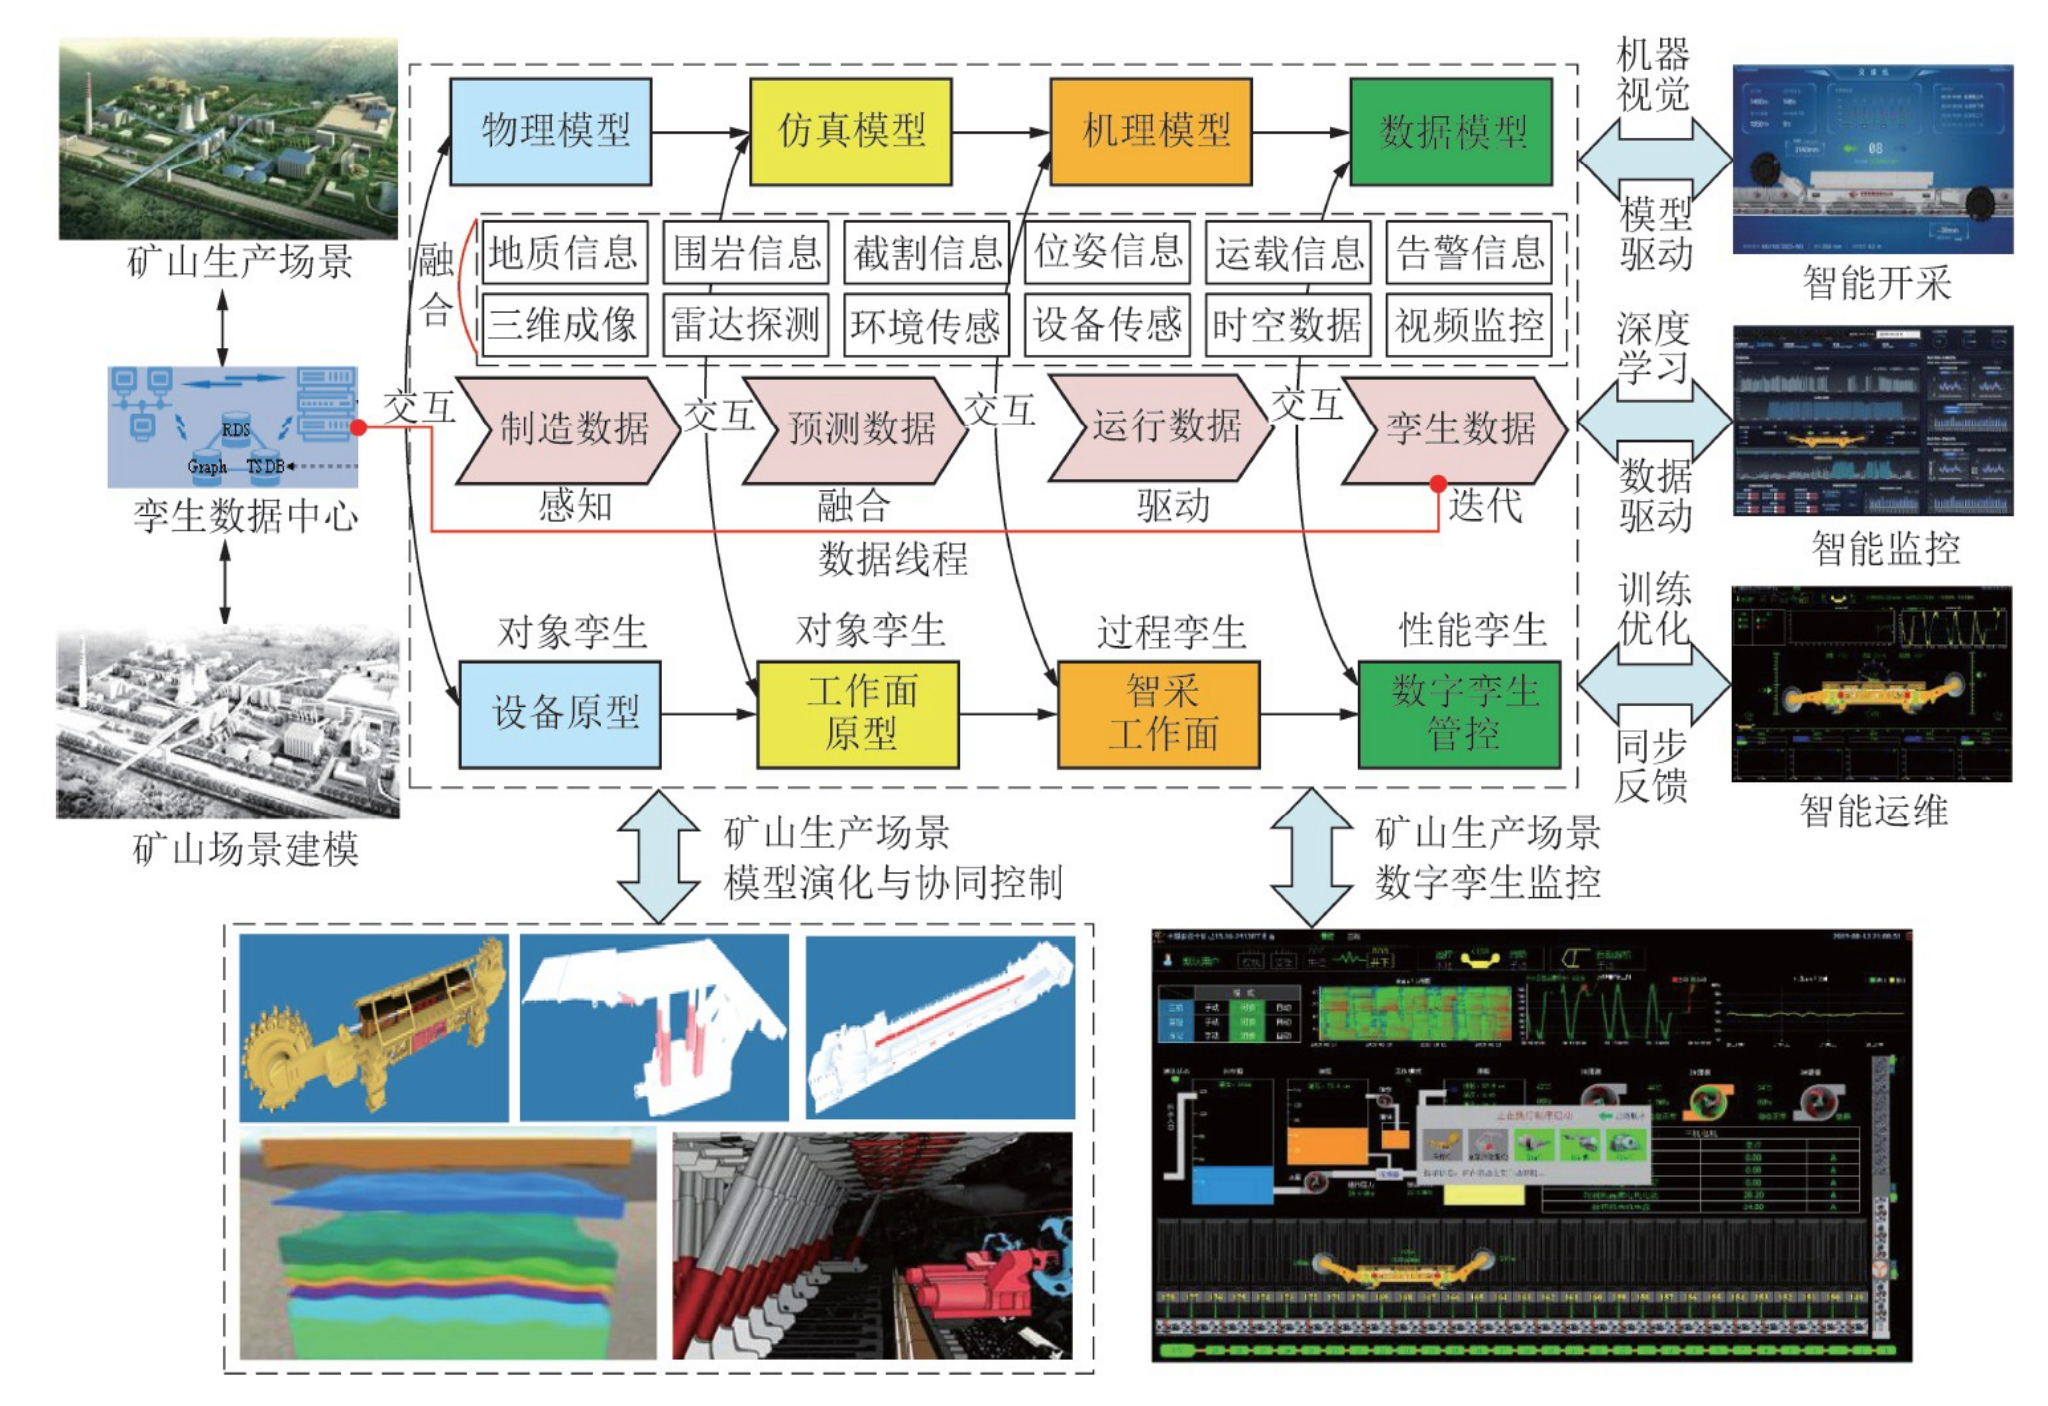
\includegraphics[width=1\textwidth]{assets/figures/1.pdf} 
    
    \caption{矿山数字孪生演化实例}
    \label{fig:pic1}
\end{figure}

\subsection{从数字孪生到平行矿山理论的演进}
在数字孪生解决物理映射准确性的基础上,如何利用虚拟空间进行前瞻性的计算实验与决策优化,成为当前研究的前沿焦点。陈龙等创新性地将复杂系统科学中的平行系统理论与人工系统、计算实验及平行执行理念引入矿山领域,正式提出了平行矿山的概念。这一概念标志着研究视角从单纯的映射孪生迈向了具备认知与推演能力的高阶智能 \citep{ChenLong_PingXingKuangShanCongShuZiLuanShengDaoKuangShanZhiNeng_2021}。平行理论强调在虚拟数字空间中构建多重演化可能的人工矿山,通过大规模计算实验推演各类极端工况下的最优控制律,进而与物理矿山进行平行交互与反馈修正。这一理论在具体的采掘业务中已展现出重要的指导意义。杨健健等基于平行执行理论构建了平行掘进系统,系统性地提出了解决掘进、支护与锚固等复杂空间交叉工序智能协同控制的理论框架 \citep{YangJianJian_PingXingJueJinJiYuACPLiLunDeJueZhiMaoZhiNengKongZhiLiLunYuGuanJianJiShu_2021}。这种从被动状态监测向主动寻优推演的理论演变,极大地拓展了智慧煤矿的应用边界。

\subsection{底层设备感知、协同控制与延伸应用}
在底层装备执行层面,工业物联网与孪生技术的融合显著提升了重型设备的运行效能与安全可靠性。丁恩杰等系统探讨了基于物联网的矿山机械设备状态智能感知与故障诊断技术。多参量光纤传感器与高精度微机电系统惯性导航等先进感知元器件的应用,为上层孪生模型提供了高维度且低延迟的时序数据馈入 \citep{DingEnJie_JiYuWuLianWangDeKuangShanJiJieSheBeiZhuangTaiZhiNengGanZhiYuZhenDuan_2023}。针对核心的综采工作面,葛世荣等提出了数字孪生智采工作面技术架构。尤秀松等进一步聚焦采煤机、刮板输送机与液压支架,提出了数字孪生驱动的群控架构,使得复杂的重型采煤装备群体能够在虚拟模型的引导下实现多机协作与运动轨迹优化 \citep{GeShiRong_ShuZiLuanShengZhiCaiGongZuoMianJiShuJiaGouYanJiu_2023, YouXiuSong_ZhiCaiGongZuoMianSanJiShuZiLuanShengQuDongKongZhiJiaGou_2024}。此外,李浩荡等将数字孪生技术与顶煤放出规律模型相协同,在提高特厚煤层资源回收率与降低混矸率方面取得了应用进展 \citep{LiHaoDang_JiYuShuZiLuanShengYuGuiHuaFangMeiXieTongDeMeiKuangZhiNengKaiCaiJiShu_2026}。智慧煤矿的技术赋能领域也在不断拓宽。李全生等将数字孪生技术下沉应用于矿区生态环境的动态监测与修复治理,构建了生态环境数字孪生的理论内涵,深刻体现了智能化开采与绿色环境保护并重的高质量发展理念 \citep{LiQuanSheng_KuangShanShengTaiHuanJingShuZiLuanShengNeiHanJiaGouYuGuanJianJiShu_2023}。


\section{研究不足}

尽管智慧煤矿与数字孪生技术在宏观架构与局部场景应用上取得了明显进展,但对标高度复杂的井下真实生产环境,现有研究与工业实践仍面临数个亟待突破的技术局限。

首先,多源异构数据的深度融合与语义对齐能力依然有限。井下工业物联网虽然接入了海量的传感器节点,但诸如地质勘探的三维点云、机电设备的震动高频频谱与环境气体的低频浓度序列等数据往往处于异构割裂状态。现有系统多采用简单的数据堆叠拼接,缺乏统一的高维特征表示机制,难以提取出支持全局协同决策的深层交叉特征。

其次,高保真物理模型与实时算力之间存在难以调和的工程矛盾。井下开采涉及非线性岩体力学损伤、瓦斯渗流以及气固液多相流体力学的复杂耦合演化。采用传统的有限元法或离散元法构建高保真物理模型需要消耗庞大的计算资源。这种计算密集型任务导致孪生系统在面对突发顶板灾害或涌水险情时,往往产生分钟级以上的计算延迟,无法做到毫秒级的实时预警与动态阻断。受限于井下有限的通信带宽,将海量原始感知数据实时上传至地面云平台进行集中求解的模式,进一步加剧了控制时延。

再次,现有分层级联控制架构对极端地质条件的泛化能力不足。目前多数智能控制策略是基于相对理想或已知的工作面条件,通过大量人工预设阈值与专家逻辑构建的。一旦工作面遭遇断层揭露、底板剧烈突水或大面积悬顶等未见异常,确定性的逻辑规则极易失效,系统依然高度依赖人工接管与经验判断,尚未实现真正的自主适应。

最后,人工智能算法在矿山安全关键系统中的可解释性与安全约束机制尚不完善。随着深度学习在矿山视觉识别与控制参数优化中的应用增多,神经网络模型内部的黑盒属性引发了工业应用的安全隐忧。在缺乏明确数学边界证明的前提下,纯数据驱动模型输出的控制指令难以满足煤矿安全规程的严苛要求,这限制了人工智能技术在核心控制闭环中的深度应用。

\section{研究趋势展望}

面向未来,破解上述数据融合困难、计算时延过高以及模型泛化泛化性差等行业痛点,需要跨界引入人工智能科学领域的前沿范式。随着通用算力集群的普及与深度学习算法的快速迭代,智慧煤矿的发展将逐步脱离传统的规则驱动路径,向具备自监督学习与主动推理能力的智能体系过渡。其主要技术演进趋势可概括为以下五个维度的拓展。

\subsection{多模态感知跃升:视觉语言模型赋能复杂场景认知}
现有的矿山视觉感知系统大多依赖于特定任务的卷积神经网络。此类判别式模型通常只能执行诸如皮带异物识别或人员轨迹追踪等特定功能,缺乏对全局场景时空关联的理解能力。未来,视觉语言大模型将在矿山感知网络中实现深度融合与应用。这类模型能够通过自注意力机制,将矿山现场的高清视频流、微光夜视图像等视觉模态,与地质勘探文本、设备维修图纸及安全操作规程等语言模态,在统一的隐空间中进行精准的语义对齐。升级后的感知系统不仅能输出异常物体的包围框坐标,更能直接理解场景上下文的物理意义。例如,当识别到采空区瓦斯浓度梯度异常且伴有煤壁温度升高时,模型可自主结合历史多尺度防灭火资料,生成自然语言形式的详细避灾路线与通风系统调节建议。这种跨模态的推理能力将显著提升孪生系统对非结构化矿山环境的通用场景认知水平。

\subsection{控制架构重构:端到端智能闭环与安全信封机制}
在采掘装备的底层执行侧,当前的控制系统普遍采用感知、决策、路径规划到动作执行的串行模块化架构 \citep{YouXiuSong_ZhiCaiGongZuoMianSanJiShuZiLuanShengQuDongKongZhiJiaGou_2024}。此架构在面对复杂工况时,容易因前端传感器的微小噪声引发后端控制参数的级联放大偏差。借鉴智能驾驶领域的前沿演进路线,端到端神经网络控制架构将成为矿机协同演进的重要方向。端到端模型直接摄入激光雷达点云与多维力矩传感器时序信号,通过深层残差网络提取时空耦合特征,并直接映射输出采煤机牵引速度、滚筒截割高度与液压支架推移步距等连续动作指令。这种方法省去了繁杂的中间规划逻辑,能够隐式学习重型装备与煤岩体之间的复杂博弈规律。为克服纯数据驱动带来的安全隐患,未来的端到端系统将普遍集成基于物理约束的安全信封机制。通过在神经网络的输出端引入反映物理极限与安全规程的可微惩罚函数,确保算法生成的所有控制指令严格收敛于煤矿安全边界之内。

\subsection{演化机理重置:世界模型驱动的生成式平行推演}
平行矿山理论的核心价值在于利用计算实验推演系统最优控制策略 \citep{ChenLong_PingXingKuangShanCongShuZiLuanShengDaoKuangShanZhiNeng_2021}。受制于微分方程求解的低效性,现有推演过程难以满足实时性要求。世界模型的引入有望为物理仿真范式带来质的飞跃。世界模型能够通过对海量历史采掘视频序列与多模态传感器信号的无监督预训练,自主内化物理世界的直观动力学规律。在实际应用中,世界模型在低维潜变量空间内以极低的算力开销,即可快速生成对矿山未来时空状态的高保真预测序列。系统无需求解纳维-斯托克斯方程或复杂岩石力学方程,即可通过神经网络快速推演未来数分钟内工作面瓦斯涌出动态或顶板位移趋势。这种生成式的计算实验使得矿山中枢大脑能够在隐空间中高效开展强化学习试错,进而将提炼出的最优参数反向映射给物理执行器,推动知识驱动与主动管控模式的真正落地 \citep{GuoYiNan_ZhiShiQuDongDeZhiCaiShuZiLuanShengZhuDongGuanKongMoShi_2023}。

\subsection{算力分布优化:云边协同与联邦学习破局数据孤岛}
针对井下数据传输的时延瓶颈,智慧矿山的算力架构正加速向云端、边缘端与设备端高度协同的分布式网络演进。部署于采煤机防爆计算机或井下变电所的高算力边缘节点,可实现传感器数据的就地近端清洗与模型推理,保障核心急停指令的毫秒级响应。此外,联邦学习机制将在跨矿区数据利用中发挥关键作用。各矿区的边缘计算集群能够在确保底层敏感生产数据不出安全域的前提下,仅将本地模型训练产生的梯度更新量加密上传至集团云端进行全局聚合。这种去中心化的协作训练模式,在兼顾数据隐私安全的同时,打破了长期存在的信息孤岛。全局大模型得以吸纳各类复杂地质条件下的运行经验,实现泛化能力的快速迭代。

\subsection{物理执行延伸:具身智能与仿生多智能体协同}
数字孪生系统的决策推演最终需要落实在物理世界的精准交互之中。传统的矿山巡检机器人多为功能单一的履带式底盘设备,缺乏在复杂受限空间内的灵巧物理作业能力。具身智能技术的快速发展将为平行矿山提供更强大的末端执行载体。未来的井下综采工作面与掘进巷道可以广泛引入具备多模态高频感知与精细力矩反馈的仿生四足机器人与双臂灵巧作业机器人。这些具身智能体能够解析系统下发的高级语义指令,并通过多智能体强化学习机制在装备群内部进行自主路径规划与任务分配。从高危区域的超前探放水钻孔定位,到狭窄管廊内的设备带电维护与管线更换,具身机器人集群将逐步胜任高强度与高风险的体力劳动环节,进而完成数字空间向物理实体改造的最终闭环。

\section{结论}

综上所述,智慧煤矿的研究已经超越了初期的单点设备自动化范畴,全面进入了以数字孪生为核心架构、以平行理论为理论指导的深水区。客观审视当前的发展阶段,在算力资源的实时优化调度、异构数据的统一语义对齐,以及极端地质条件下的模型泛化验证等方面,工业界与学术界仍面临诸多严峻的工程与理论挑战。

应对上述挑战,跨学科融合创新是必由之路。从视觉语言大模型带来的全场景深度认知,到端到端控制架构实现的鲁棒闭环,再到世界模型赋予数字孪生的超实时预测能力,叠加边缘计算与具身智能的协同发展,新一代计算机科学技术的融合应用为智慧煤矿的升级提供了全新的解题思路。这些技术的逐步落地,将推动智慧煤矿从机械的物理状态复刻向具备自主进化能力的工业大脑演进。建立高可靠、强泛化的智能平行矿山体系,不仅是实现煤炭资源安全高效开采的必然选择,更是推动煤炭工业向低碳环保与可持续发展转型的重要基石。

% \newpage
% \printbibliography[heading=bibintoc, title=参考文献]
